\documentclass[12pt,a4paper,onecolumn]{article}


\usepackage[utf8]{inputenc}
\usepackage[french]{babel}
\usepackage[T1]{fontenc}
% \usepackage{amsmath}
% \usepackage{amsfonts}
% \usepackage{amssymb}
\usepackage{graphicx}
\usepackage[left=2cm,right=2cm,top=2cm,bottom=2cm]{geometry}
% \usepackage{lipsum}
\usepackage{multicol}
\usepackage{float}
\usepackage{comment}
\usepackage{hyperref}

\author{Anthony \bsc{Lhopital} \and Baptiste \bsc{Rouger}}
\title{Étude de l'intéraction symbiotique entre \textit{Aeschynomene indica} et trois souches de \textit{Bradyrhizobium sp.} ORS285 dans différentes conditions de concentrations de KNO3 et de NaCl.}

\begin{document}

	\maketitle

	\paragraph{Mots-clés :}
	\textit{Bradyrhizobium sp.} ORS285, \textit{Aeschynomene indica}, bclA, symbiose


	\begin{abstract}
		L'étude des différentes intéractions entre \textit{Aeschynomene indica} et les trois souches de \textit{Bradyrhizobium sp.} ORS285 sous différentes concentrations de NaCl et de KNO3 ont montré que la présence d'une des souches suffisait pour induire une nodulation. Toutefois, la souche C ne semble pas fixer l'azote, ou très peu par rapport aux deux autres souches. L'étude de la souche B sous différentes conditions, soit de stress salin, soit en supplément de KNO3, a montré une diminution du nombre de nodulations quand on augmente la concentration et à 50mM de KNO3 et 75mM de NaCl, une absence de nodules. En parallèle, l'appareil caulinaire avait tendance à être plus développé que l'appareil racinaire.


	\end{abstract}


	\begin{multicols}{2}


		\section{Introduction}

			La coévolution de \textit{Aeschynomene indica} et \textit{Bradyrhizobium sp.} a mené à une symbiose des deux espèces. Cette symbiose Rhyzobium-Légumineuse est l'un des meilleurs exemples d'apport symbiotique d'azote dans le milieu pour les plantes. L'étude de ce phénomène, tant d'un point de vue physiologique que génomique, permettrait de mieux l'appréhender, ce qui permettrait de grandes avancées dans les domaines théoriques de la symbiose comme dans l'amélioration possible de plantes non-symbiotiques dépendantes de l'azote vers une espèce modifiée qui pourrait pratiquer une symbiose du même type que  celle de \textit{Aeschynomene indica} et \textit{Bradyrhizobium sp.}. Dans ce but, nous avons utilisé une approche anatomique de cette symbiose pour déterminer les effets de différentes conditions et de différentes souches sur cette symbiose.

		\section{Matériels et méthodes}

			L’étude de la symbiose Rhizobium-Légumineuses se fait entre \textit{Aeschynomene indica} et trois souche de \textit{Bradyrhizobium sp.} ORS285 : souche sauvage (A), souche pnifH::gus (B) et une souche mutante bclA (C).\\

			Les plantes ont été placées en culture le jour à 27\degre C et la nuit à 20\degre C la première semaine après inoculation, au lieu de 28\degre C et à 57\% HR au lieu de 80\%.


		\section{Résultats}

			8 jours après inoculation avec les différentes souches et concentration de KNO3 et NaCl, l’observation (\textsc{Figure}~\ref{taille8}) du phénotype des plantes non inoculées et sans ajout de NaCl ou de KNO3 ont des cotylédons jaunes et avec 2 à 3 étages foliaires. Les plantes non inoculées avec un ajout de KNO3 ont montré une croissance plus élevée avec des cotylédons verts et entre 3 et 6 étages foliaires. Pour les plantes inoculées avec la souche A, on observe entre 2 et 3 étages foliaires et les cotylédons de couleur verte alors que les plantes inoculées avec la souche C ont des cotylédons jaunes. Pour les plantes inoculées avec la souche B, les cotylédons sont verts et on compte entre 2 et 3 étages foliaires sans ajout de KNO3 et 1 voir 2 étages de plus avec un ajout de KNO3.

			% \begin{figure}[H]
			% 	\begin{center}
			% 		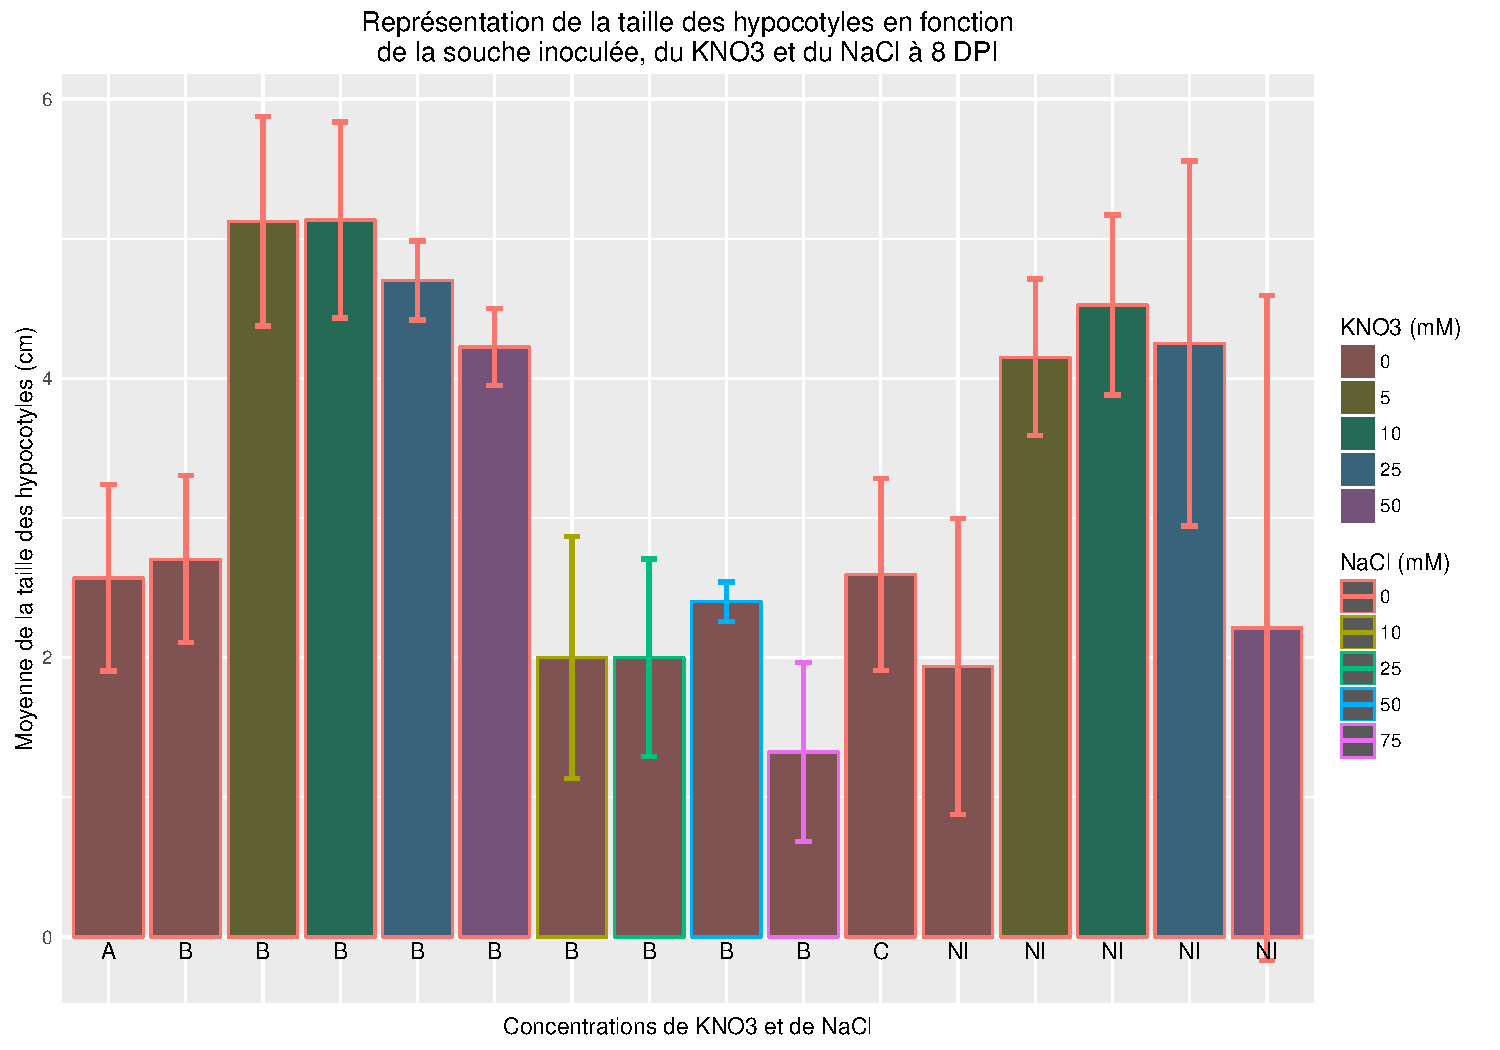
\includegraphics[width=\linewidth]{taille8.pdf}
			% 	\end{center}
			% 	\caption{Taille de l’appareil caulinaire en fonction de la souche inoculée, de KNO3 et du NaCl à 8 DPI (NI : non inoculée, A, B et C : inoculation avec la souche  A, B et C)}
			% 	\label{taille8}
			% \end{figure}

			Les mesures de l’appareil caulinaire montrent qu’une plante non inoculée a une taille variable en fonction de la concentration de KNO3 dans le milieu. A une concentration de O mM, l'appareil caulinaire mesure une moyenne de 2 cm. Pour des concentrations de KNO3 de 5, 10 et 25 (mM), on observe (\textsc{Figure}~\ref{taille8}) des tailles moyennes de 2.4cm. De plus, les inoculations avec les trois souches sans KNO3 montrent une taille semblable, soit de 2.5cm. Les plantes inoculées avec la souche B avec un apport de KNO3 montrent une croissance deux fois plus élevée quelque soit la concentration alors qu’en présence de NaCl on observe une croissance plus faible (2cm) pour les concentrations de 10, 25 et 50mM et à 75mM on observe une taille de 1.5cm.

			% \begin{figure}[H]
			% 	\begin{center}
			% 		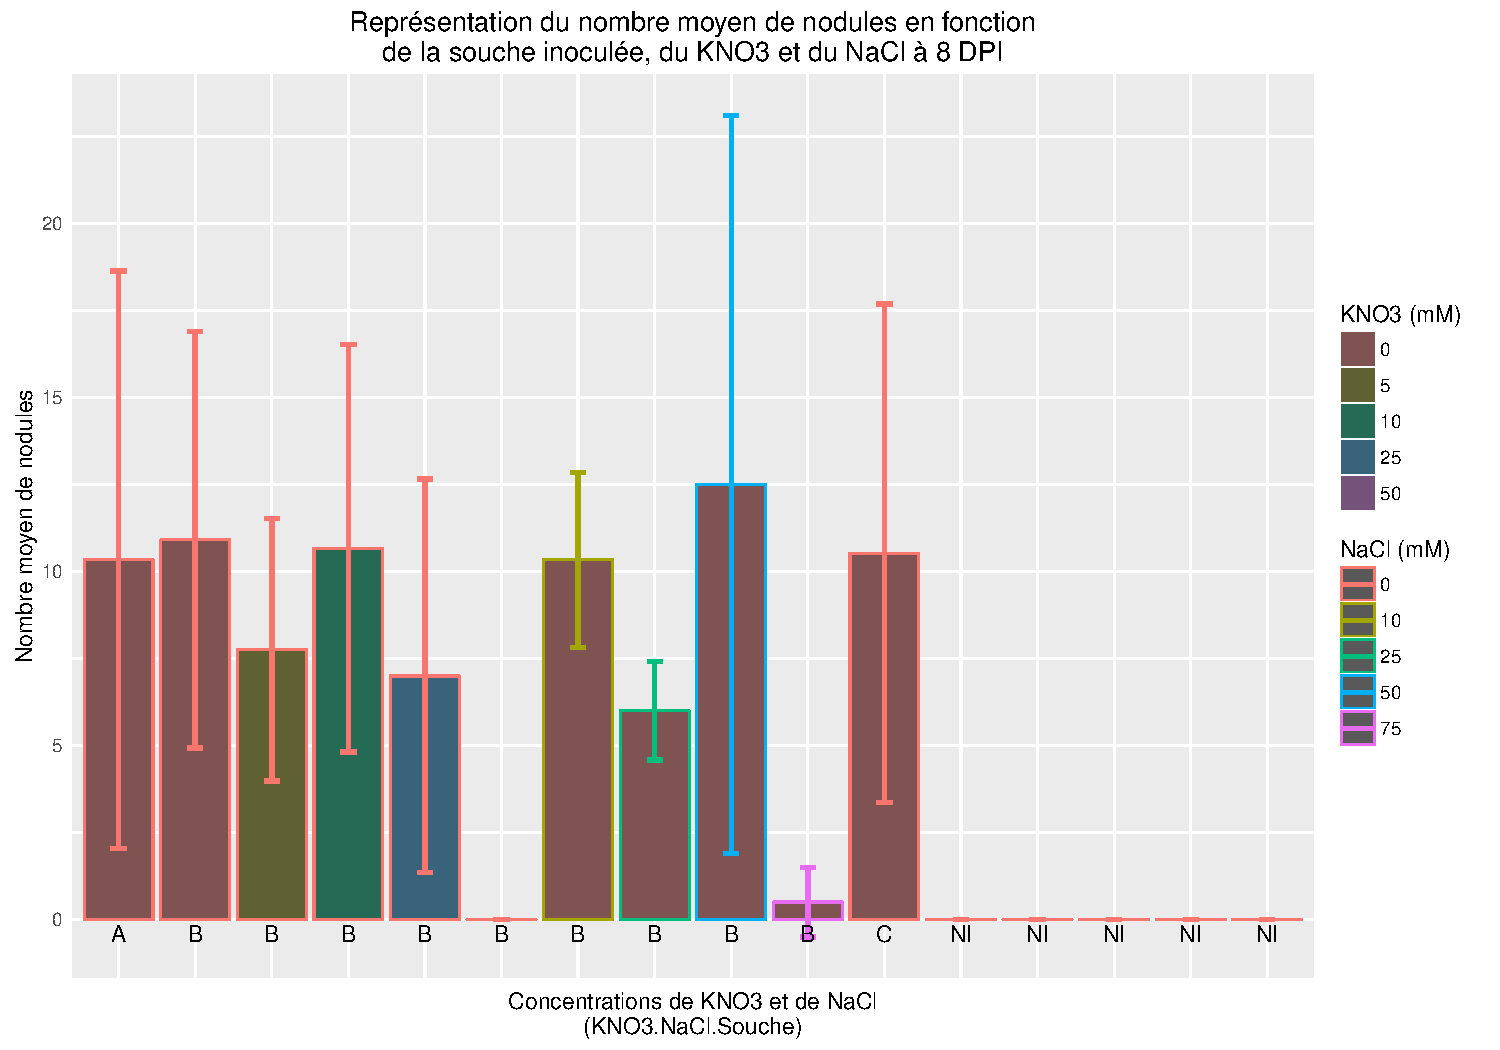
\includegraphics[width=\linewidth]{nodmean8.pdf}
			% 	\end{center}
			% 	\caption{Nombre moyen de nodules en fonction de la souche inoculée, du KNO3 et du NaCl à 8DPI (NI : non inoculée, A, B et C : inoculation avec la souche  A, B etC)}
			% 	\label{nodmean8}
			% \end{figure}

			On observe (\textsc{Figure}~\ref{nodmean8}) une absence de nodulation pour les plantes non inoculées ainsi que pour des fortes concentrations de NaCl (75mM) ou de KNO3 (50mM). Pour les différentes souches, on observe une moyenne de 11 nodules sans ajout de NaCl ou de KNO3. L’ajout de KNO3 pour les plantes inoculées avec la souche B, présentent en moyenne 8 nodules pour des concentrations de  5 à 25mM. L’ajout de NaCl montre des résultats similaires pour des concentrations de 25 à 75mM et à 10mM : on compte en moyenne 10 nodules.

			% \begin{figure}[H]
			% 	\begin{center}
			% 		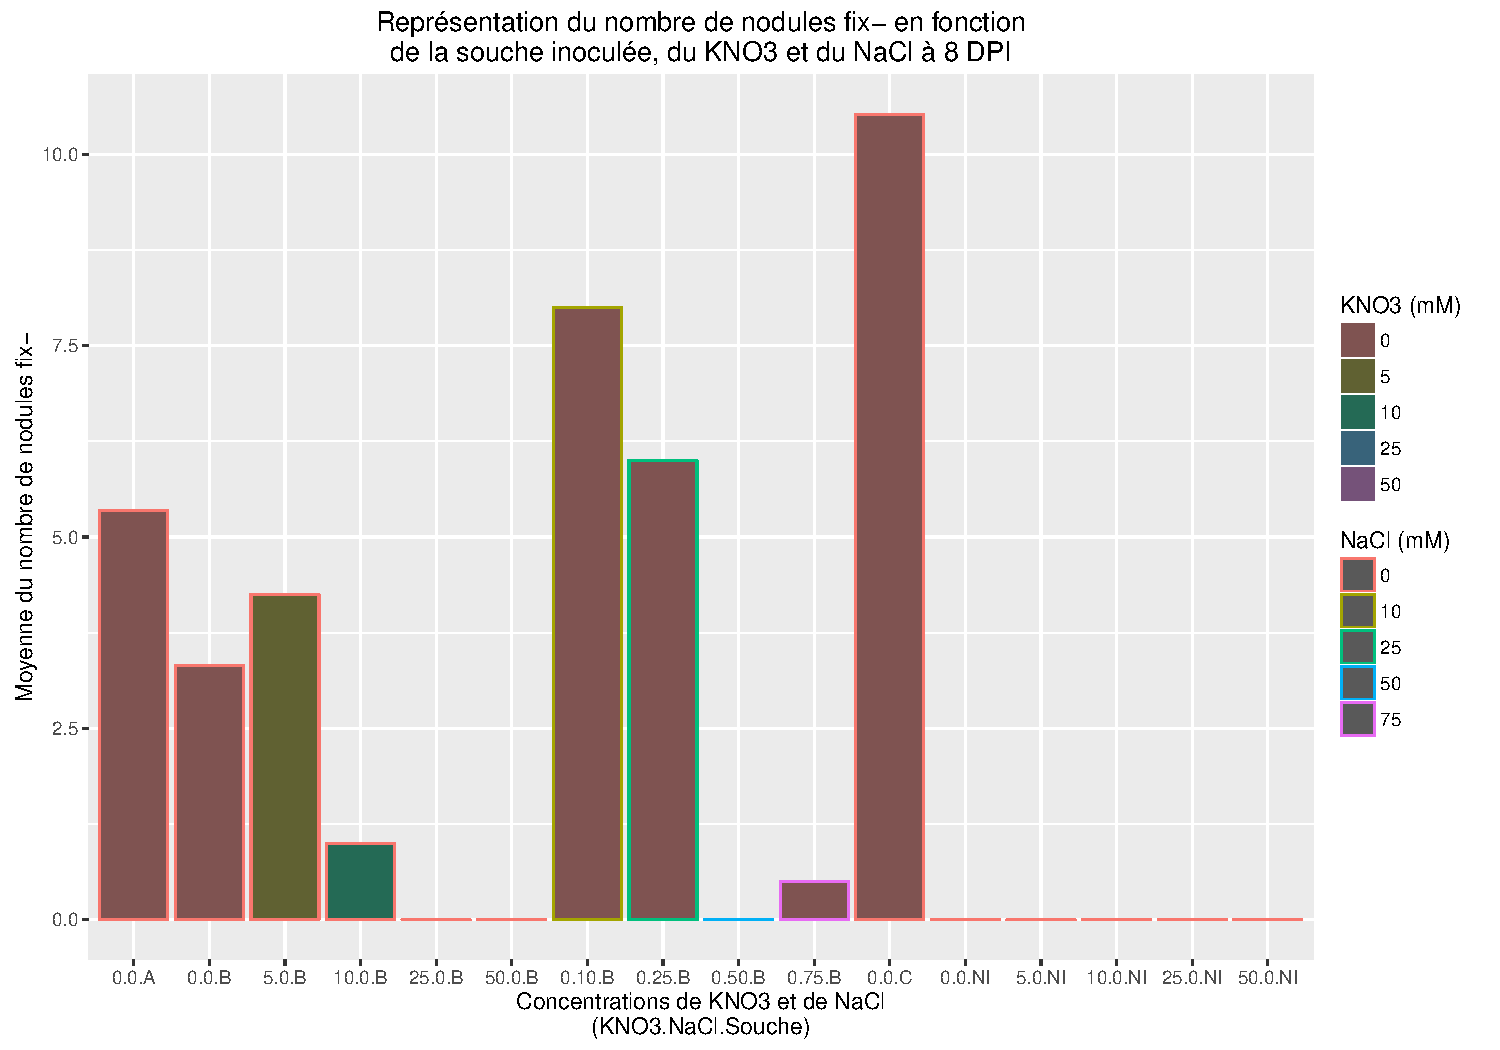
\includegraphics[width=\linewidth]{nod-mean8.pdf}
			% 		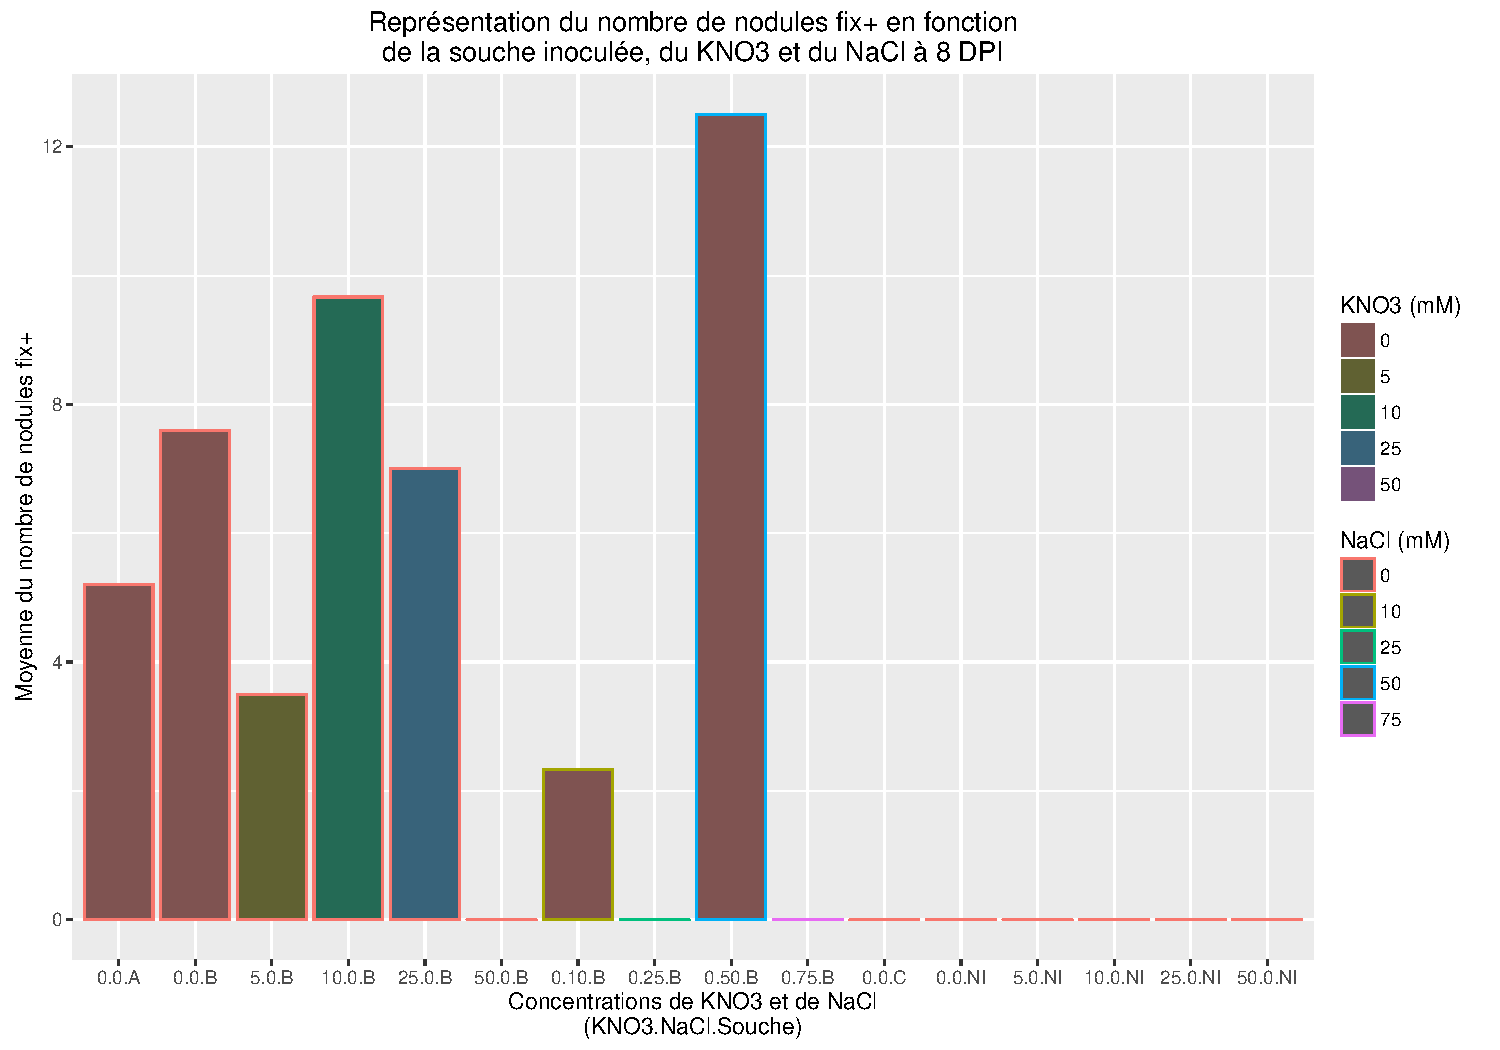
\includegraphics[width=\linewidth]{nod+mean8.pdf}
			% 	\end{center}
			% 	\caption{Nombre moyen de nodules fixateurs (fix+) ou non (fix-) d’azote en fonction de la souche inoculée, de KNO3 et du NaCl à 8 DPI}
			% 	\label{fix+-8}
			% \end{figure}

			L’observation (\textsc{Figure}~\ref{fix+-8}) de la couleur des nodosités a permis d'identifier celles qui étaient susceptibles de fixer l’azote.  On observe à 8DPI que les inoculations avec la souche C n’ont donné aucune nodosités fixatrices d’azote. Pour les inoculations avec la souche B en présence de KNO3, on observe plus de nodosités fixatrices quand la concentration augmente. En présence de NaCl, on observe le même phénomène, sauf à 25mM de NaCl où l'on observe aucune nodosité fixatrice. De plus, on observe que les plantes inoculées avec la souche A ont 50\% de leurs nodosités fixatrices d’azote. Pour les fortes concentration de NaCl (75mM) et de KNO3 (50mM) et les plantes non inoculées, on a une absence complète de nodosités d’où l’absence de barre sur le graphe.




			% \begin{figure}[H]
			% 	\begin{center}
			% 		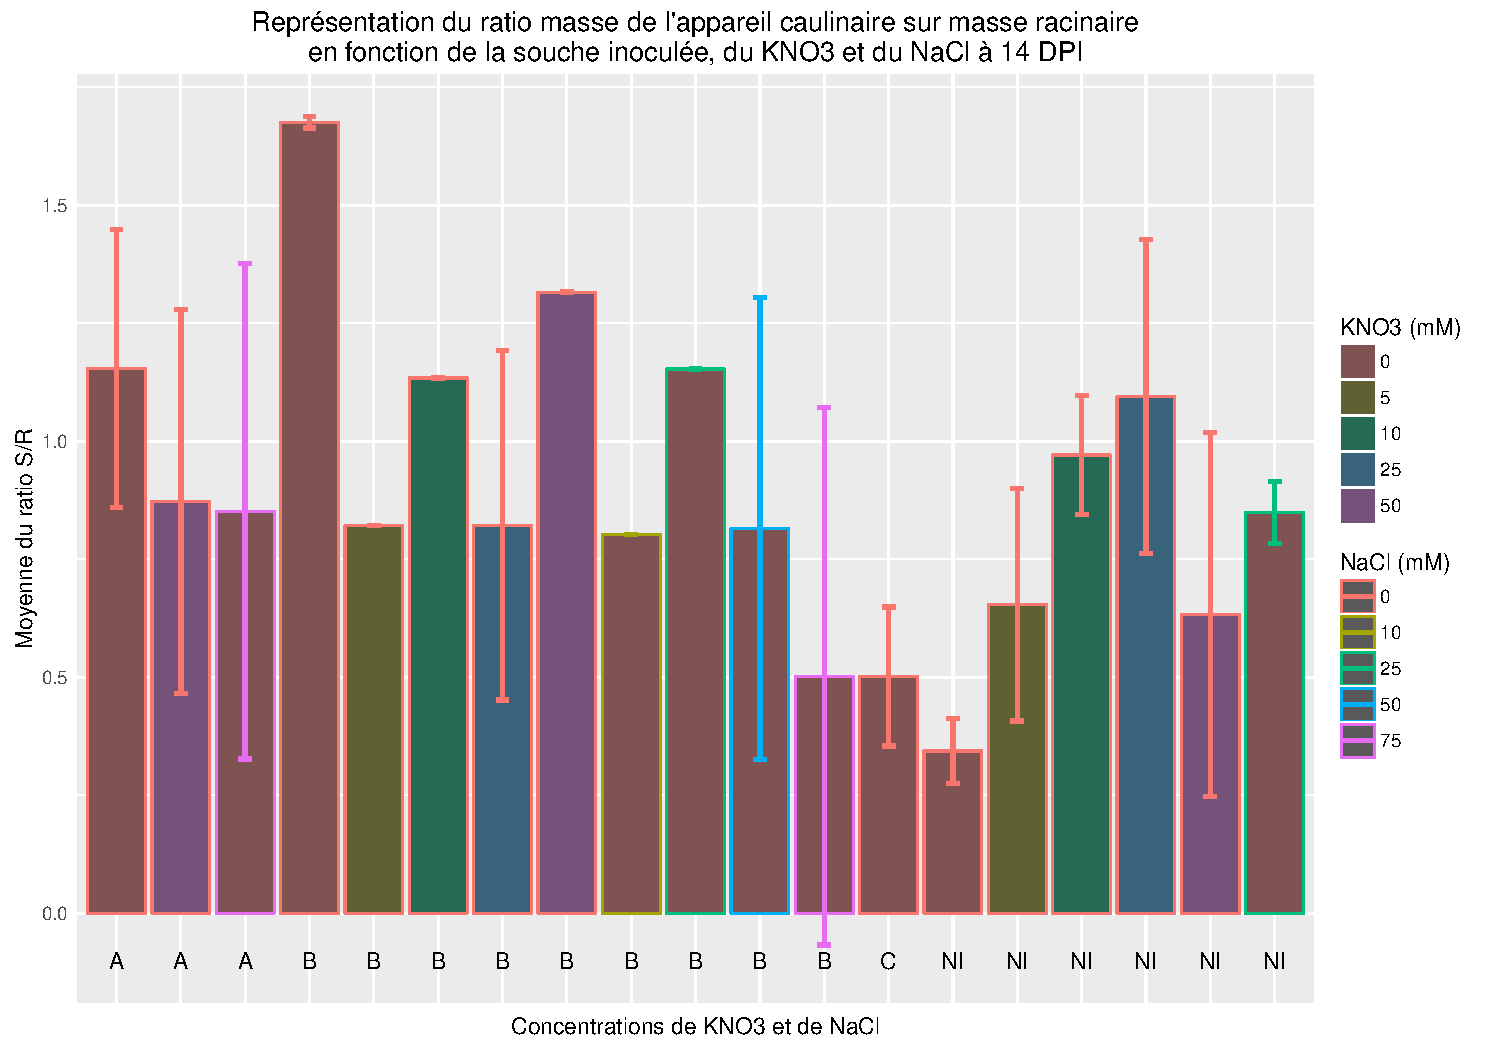
\includegraphics[width=\linewidth]{SR14.pdf}
			% 	\end{center}
			% 	\caption{Ratio entre la masse de l’appareil caulinaire et l’appareil racinaire en fonction  de la souche inoculée, de KNO3 et du NaCl à 14 DP}
			% 	\label{SR14}
			% \end{figure}

			On observe (\textsc{Figure}~\ref{SR14}) à 14DPI une croissance plus élevée de l’appareil caulinaire par rapport à l’appareil racinaire allant presque jusqu'à un facteur 2 dans l’inoculation avec la souche B. Les plantes non inoculées ont une croissance caulinaire plus élevée par rapport à l’appareil racinaire quand on ajoute du KNO3 (entre 0.75 et 1.2) alors que sans cet apport on observe un rapport de 0.4. Les plantes non inoculées et mises en présence de NaCl à une concentration de 25mM montrent un ratio de la masse de 0.8. De plus, on observe chez les inoculations avec la souche A, un ratio de 1.2 sans aucun ajout et un ratio plus faible (0.8) en présence de NaCl ou de KNO3. Quant aux inoculations avec la souche C, on observe un ratio de 0,5. Pour les plantes inoculées avec la souche B on observe qu’avec un apport de KNO3 le ratio augmente mais est inférieur aux plantex sans apport (0.8 à 1.3). Alors qu’en présence de NaCl, on observe une diminution du ratio quand la concentration augmente, c'est-à-dire une diminution de 1,8 à 0,7.

			% \begin{figure}[H]
			% 	\begin{center}
			% 		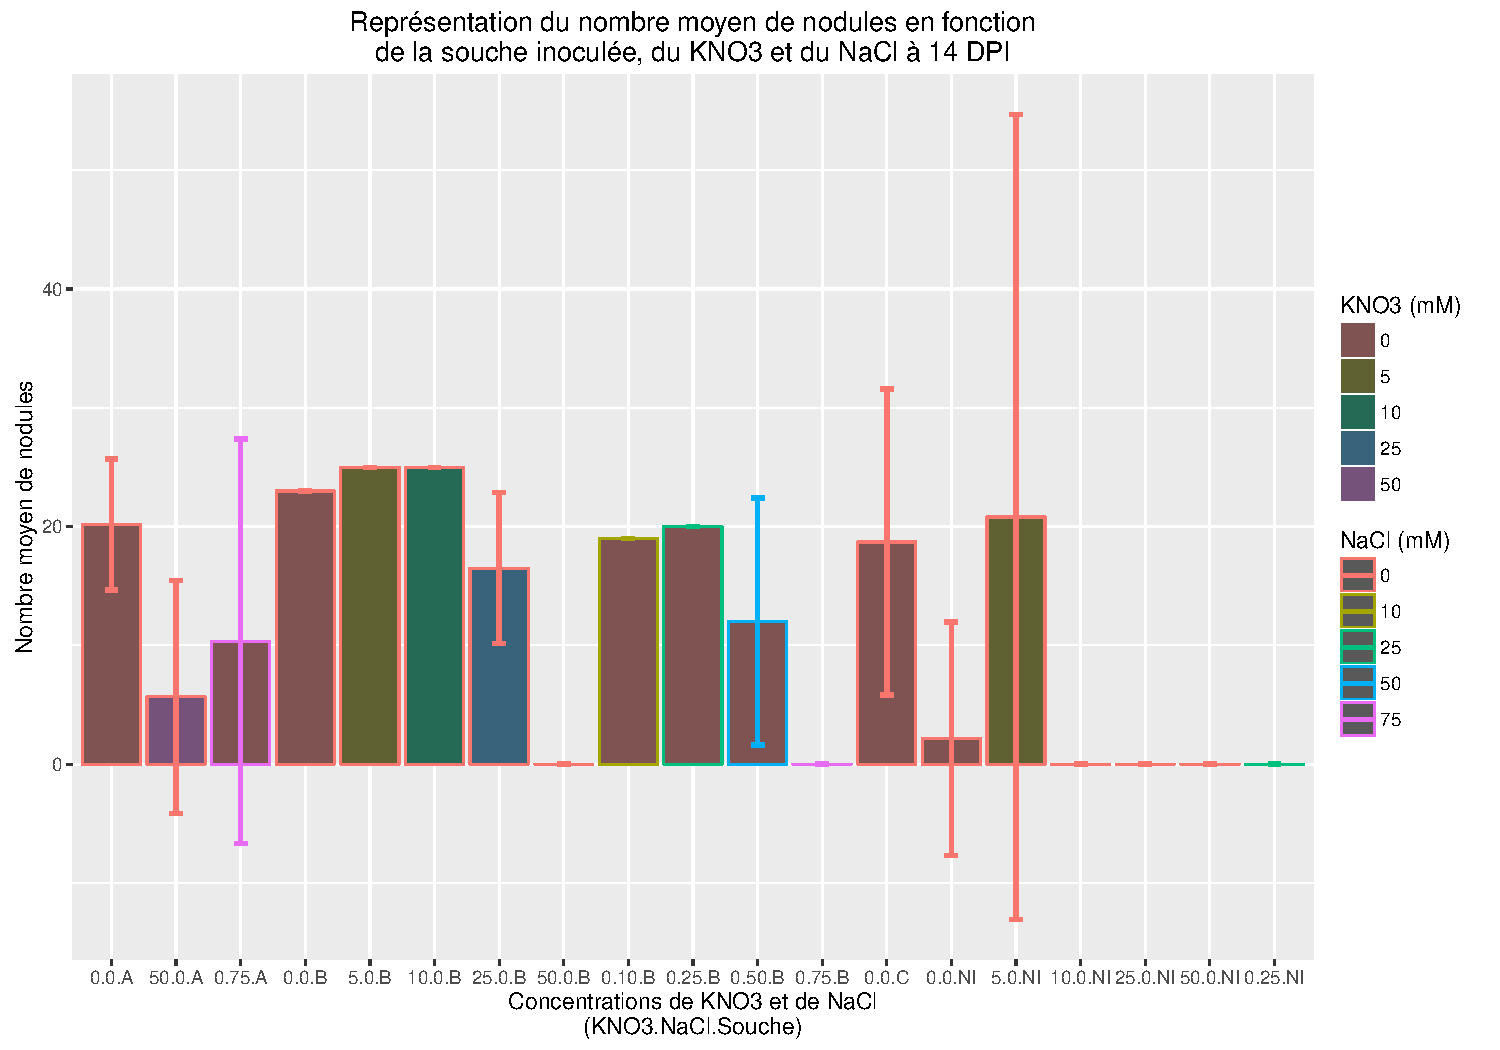
\includegraphics[width=\linewidth]{nodmean14.pdf}
			% 	\end{center}
			% 	\caption{Nombre moyen de nodules en fonction de la souche inoculée, du KNO3 et du NaCl à 14DPI (NI : non inoculée, A, B et C : inoculation avec la souche  A, B et C)}
			% 	\label{nodmean14}
			% \end{figure}

			On observe (\textsc{Figure}~\ref{nodmean14}) une absence de nodulation pour les plantes non inoculées quelque soit la concentration de KNO3 ajoutée. Pour l’inoculation avec la souche C, on observe en moyenne 16 nodules. Pour la souche A, on observe une moyenne de 18 nodules sans ajout de KNO3 ou de NaCl et une diminution du nombre de nodules en présence d’une forte concentration de KNO3 ou NaCl, respectivement 6 et 10 nodules. Pour la souche B, on observe en moyenne 23 nodules sans ajout de KNO3 et NaCl et on observe une diminution du nombre de nodules quand la concentration en KNO3 augmente. De plus, on observe plus de nodules pour des concentrations de 10mM de NaCl, soit de 32 nodules, ainsi qu’une diminution du nombre de nodules pour des concentrations plus fortes de NaCl.


			% \begin{figure}[H]
			% 	\begin{center}
			% 		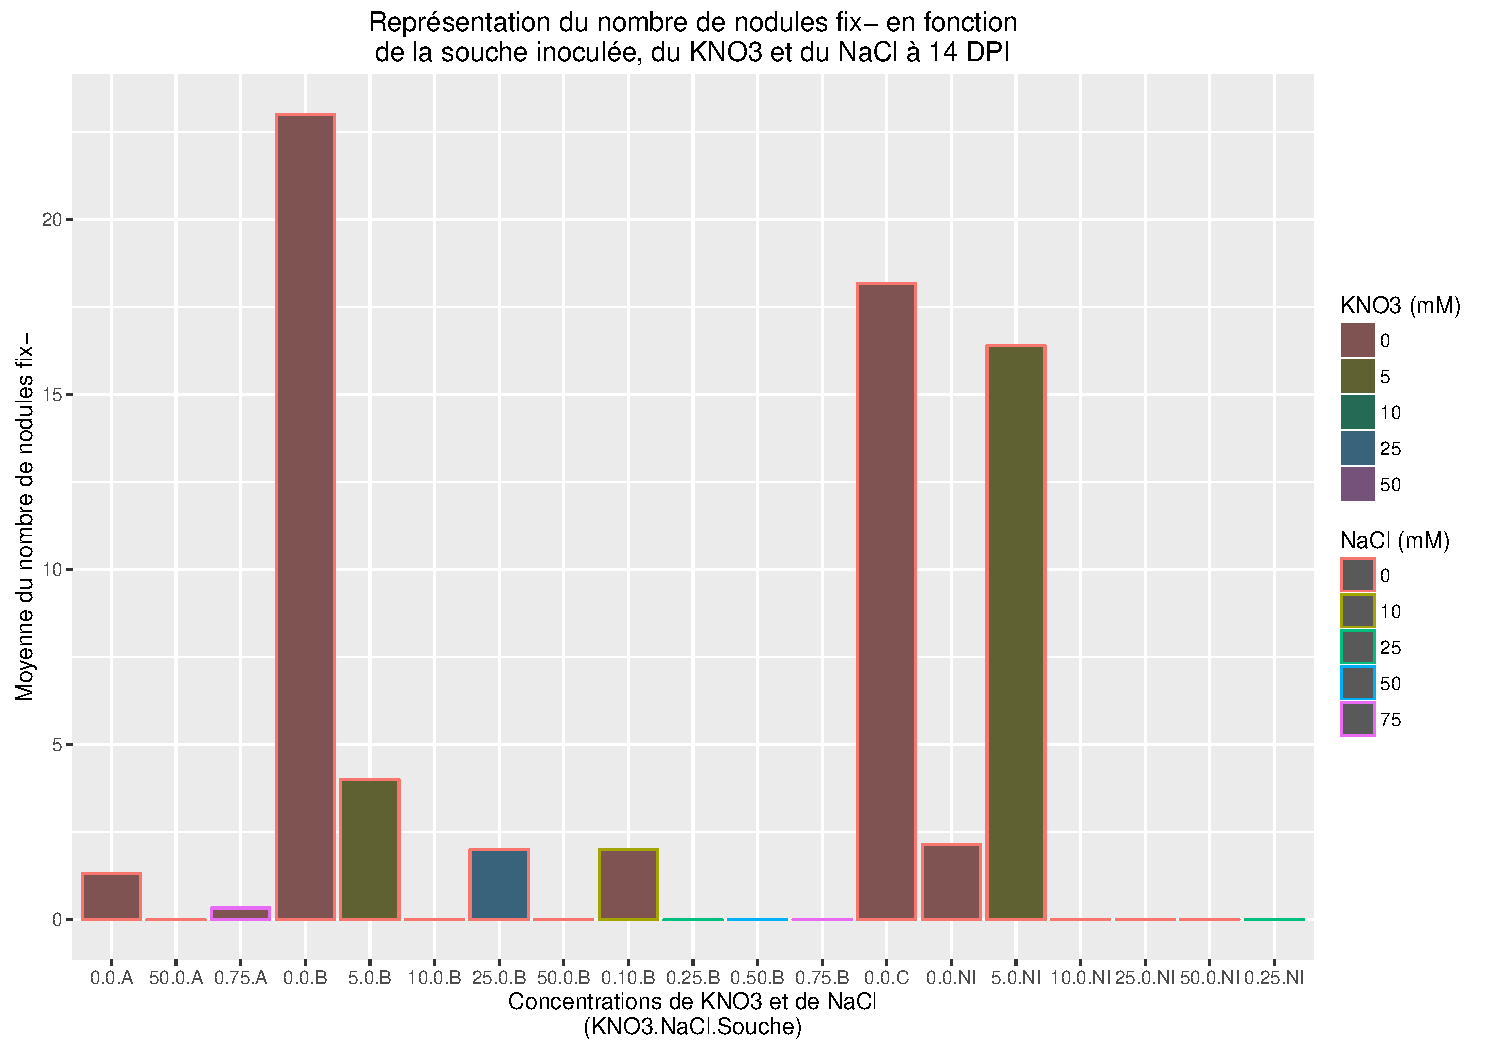
\includegraphics[width=\linewidth]{nod-mean14.pdf}
			% 		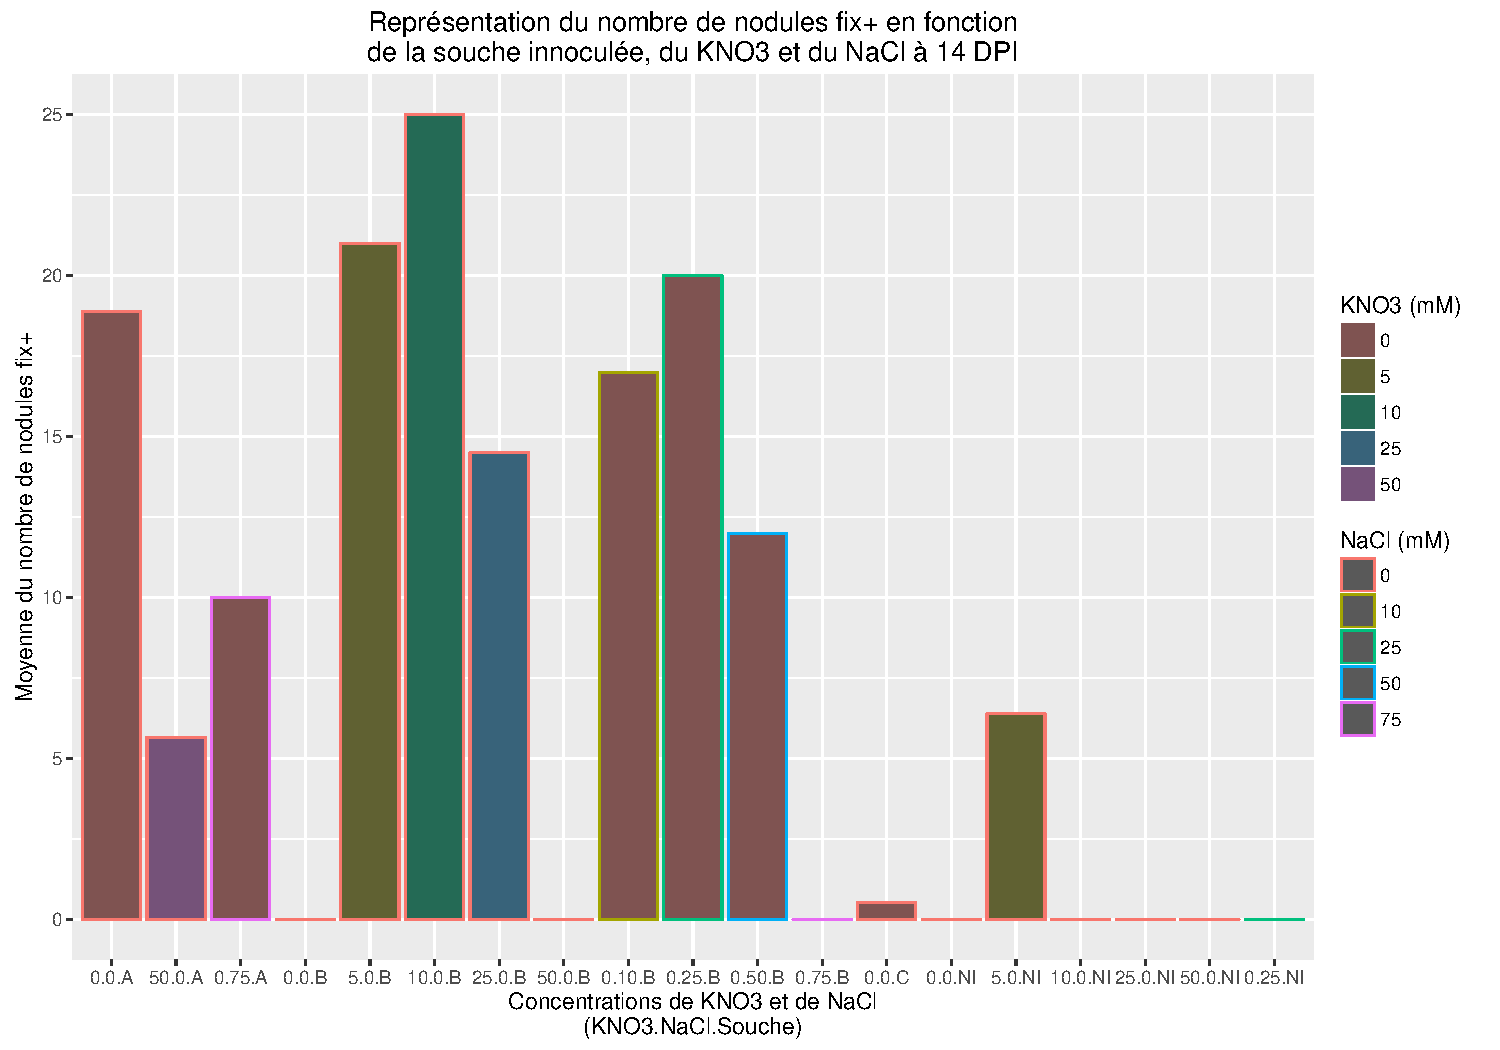
\includegraphics[width=\linewidth]{nod+mean14.pdf}
			% 	\end{center}
			% 	\caption{Nombre moyen de nodules fixateurs (fix+) ou non (fix-) d’azote en fonction de la souche inoculée, de KNO3 et du NaCl à 14 DPI}
			% 	\label{fix+-14}
			% \end{figure}

			À 14DPI, on observe (\textsc{Figure}~\ref{fix+-14}) que les plantes inoculées avec la souche C ont peu de nodosités fixatrices d’azote, alors que les inoculations avec les souches A et B montrent une fixation de l’azote dans quasiment toutes les nodosités formées. De plus, on observe chez les plantes inoculées avec la souche B, alors qu’en absence de NaCl ou de KNO3 ainsi qu'en très forte concentration, soit à 50mM de KNO3, soit 75mM de NaCl, on n’a pas de nodules fixateurs d’azote. Pour les plantes non inoculées, on a une absence complète de nodosités d’où l’absence de barre sur le graphe.


			L’observation au microscope des bactéries contenues dans les nodosités, avaient des formes et tailles différentes de la souche de référence sauvage. En effet, celle-ci mesure environ 1$\mu$m de longueur et avaient une forme de bâtonnet. Or, les souches A et B avaient une forme circulaire et faisaient environs 2.5$\mu$m de diamètre. Quant à la souche C, il y avait un mélange de bactéries en forme de bâtonnet et de forme sphérique, dont la taille était proche de la souche sauvage.

			\section{Discussion}

			On a cherché à déterminer quel était l’impact dû au sel et au nitrate sur la mise en place de la nodulation chez \textit{Aeschynomene indica} ainsi que son fonctionnement en présence ou non de \textit{Bradyrhizobium sp.}. De plus, on a cherché à déterminer l’impact que pouvait avoir une mutation de bclA chez cette bactérie sur la symbiose Rhizobium-Légumineuse.

			La mise en place de la nodulation mise en évidence à 8DPI, montre un besoin de la présence de \textit{Bradyrhizobium sp.} pour se mettre en place. En effet, pour les plantes non inoculées, on a une absence de nodulation alors que les plantes inoculées avec les différentes souches de la bactéries ont toutes formé des nodosités. De plus, la présence de NaCl ou de KNO3 semble jouer un rôle dans la formation de nodules. Avec une concentration plus élevée en NaCl ou en KNO3, le nombre de nodosités diminue. De plus, le KNO3 semble favoriser la croissance des plantes. Celles-ci présentaient entre 1 et 3 étages foliaires supplémentaires et ne semblaient pas avoir puisé dans leurs réserves stockées dans les cotylédons, tandis que les plantes non inoculées et sans ajout de KNO3 comptaient entre 2 et 3 étages foliaires et avaient des cotylédons jaunes voire même perdus. Ceci diffère des plantes inoculées avec les souche A et B : la croissance est similaire mais les cotylédons sont verts et pour la souche C les cotylédons sont jaunes voire perdus. Cette première observation montre qu’il y a eu un effet des bactéries de la souche A et B sur la croissance de la plante. Par la suite, l’observation de la couleur des nodules nous permet de déterminer celles qui étaient susceptibles de fixer l’azote. En corrélation avec le phénotype des plantes inoculées, celles mises en présence de la souche C, semblaient n'avoir aucune nodosité fixatrice d’azote alors que celles inoculées avec les souches A et B présentaient au moins 50\% de nodules fixateurs d’azote. Ceci pourrait expliquer pourquoi la présence de ces nodules engendre un phénotype semblable aux plantes non inoculées dont le milieu était supplémenté en KNO3. La présence de KNO3 ou de NaCl à des concentrations croissantes montre que le nombre de nodosités fixatrices augmente jusqu’à des concentrations de 25mM de KNO3 et 50mM de NaCl. À 50mM de KNO3 et75mM de NaCl, on a observé une absence de nodosités, ce qui montre qu’à de hautes concentrations, la nodulation ne se met pas en place. On peut supposer qu’une très forte concentration de KNO3 permet à la plante de subvenir de manière efficace à ses besoins et rend donc la nodulation inutile. Quant au NaCl, une forte concentration entraîne un fort stress salin ce qui pourrait être la cause du phénotype anormal des plantes.\\
			Nous avons donc vu les conséquences anatomiques de différentes conditions et souches de \textit{Aeschynomene indica} sur la symbiose en cette dernière et \textit{Bradyrhizobium sp.}. Il serait à présent intéressant d'essayer de localiser tous les gènes indispensables à cette symbiose pour en faire un modèle complet.

		\end{multicols}

		\newpage

		\begin{figure}[p]
			\begin{center}
				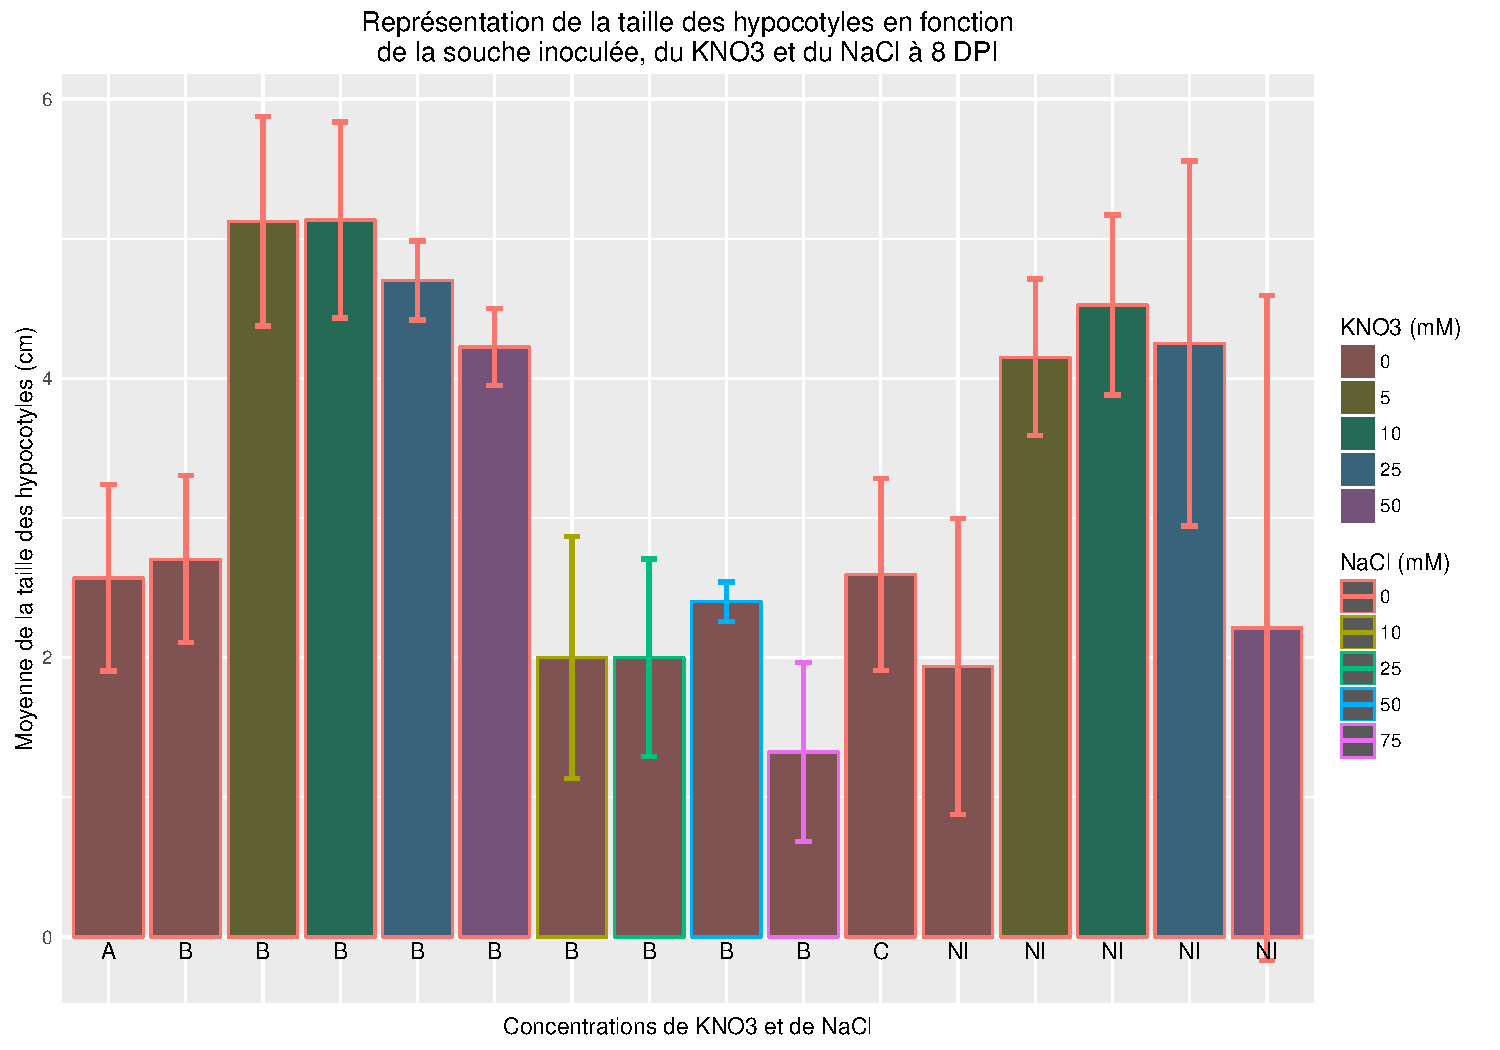
\includegraphics[width=0.9\linewidth]{taille8.pdf}
			\end{center}
			\caption{Taille de l’appareil caulinaire en fonction de la souche inoculée, de KNO3 et du NaCl à 8 DPI (NI : non inoculée, A, B et C : inoculation avec la souche  A, B et C)}
			\label{taille8}
		\end{figure}

		\begin{figure}[p]
			\begin{center}
				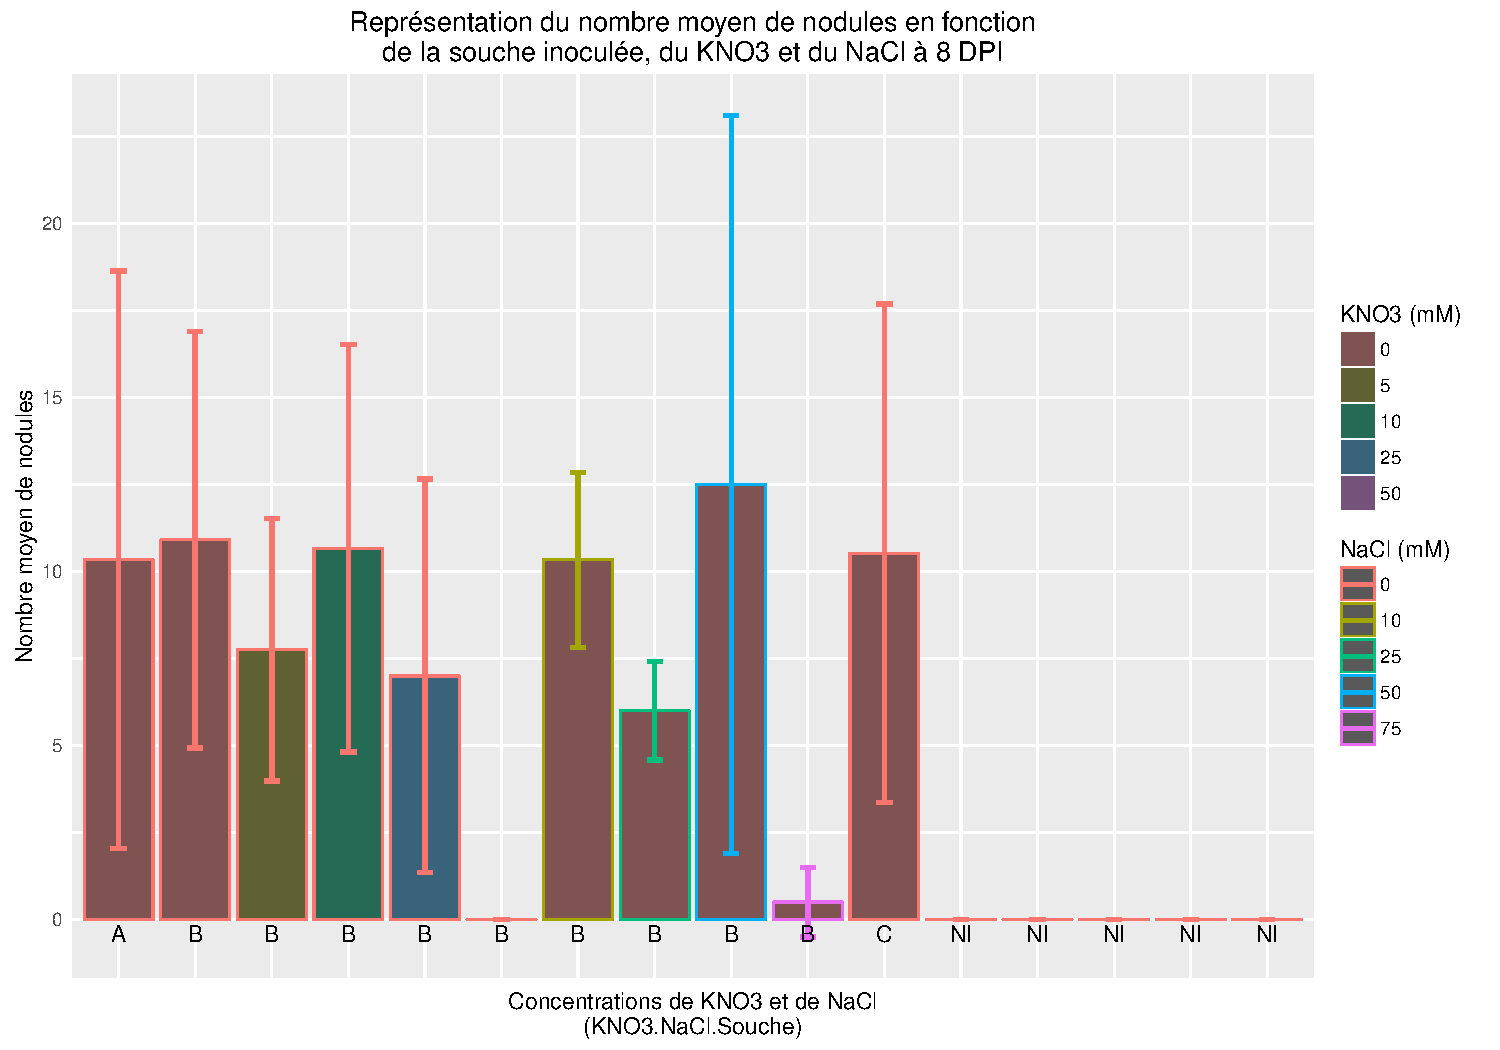
\includegraphics[width=0.9\linewidth]{nodmean8.pdf}
			\end{center}
			\caption{Nombre moyen de nodules en fonction de la souche inoculée, du KNO3 et du NaCl à 8DPI (NI : non inoculée, A, B et C : inoculation avec la souche  A, B etC)}
			\label{nodmean8}
		\end{figure}


		\begin{figure}[p]
			\begin{center}
				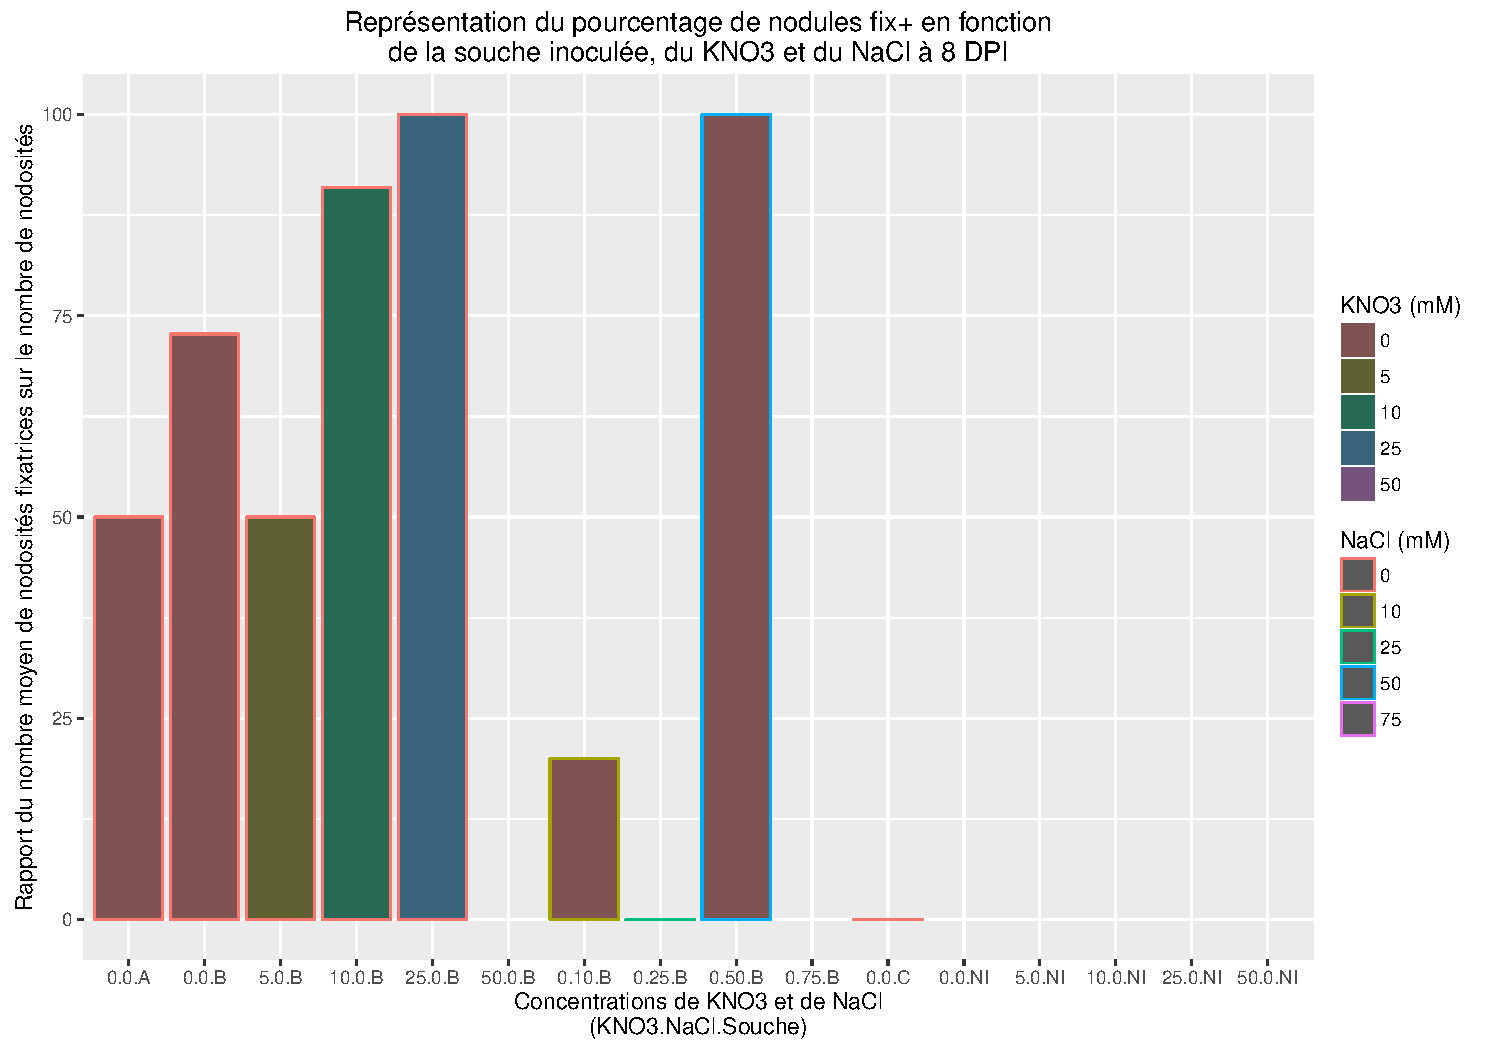
\includegraphics[width=0.9\linewidth]{rapfix+nod8.pdf}
			\end{center}
			\caption{Pourcentage de nodule fixatrice d’azote en fonction de la souche inoculée, de KNO3 et du NaCl à 8 DP}
			\label{fix+-8}
		\end{figure}

		\begin{figure}[p]
			\begin{center}
				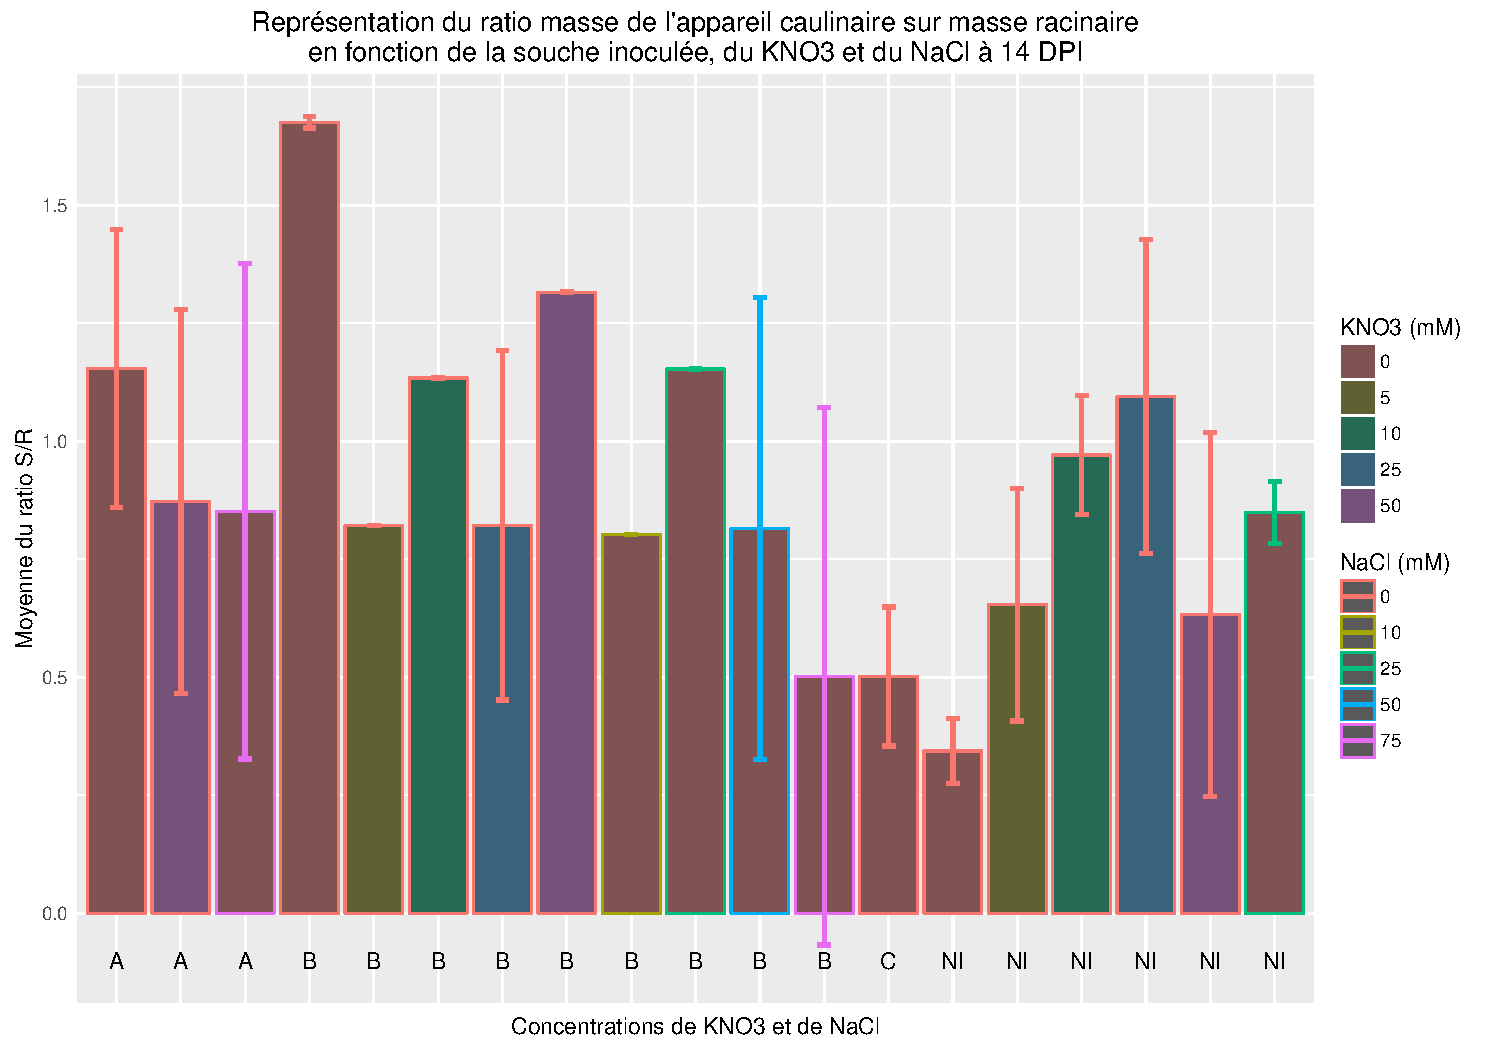
\includegraphics[width=0.9\linewidth]{SR14.pdf}
			\end{center}
			\caption{Ratio entre la masse de l’appareil caulinaire et l’appareil racinaire en fonction  de la souche inoculée, de KNO3 et du NaCl à 14 DP}
			\label{SR14}
		\end{figure}

		\begin{figure}[p]
			\begin{center}
				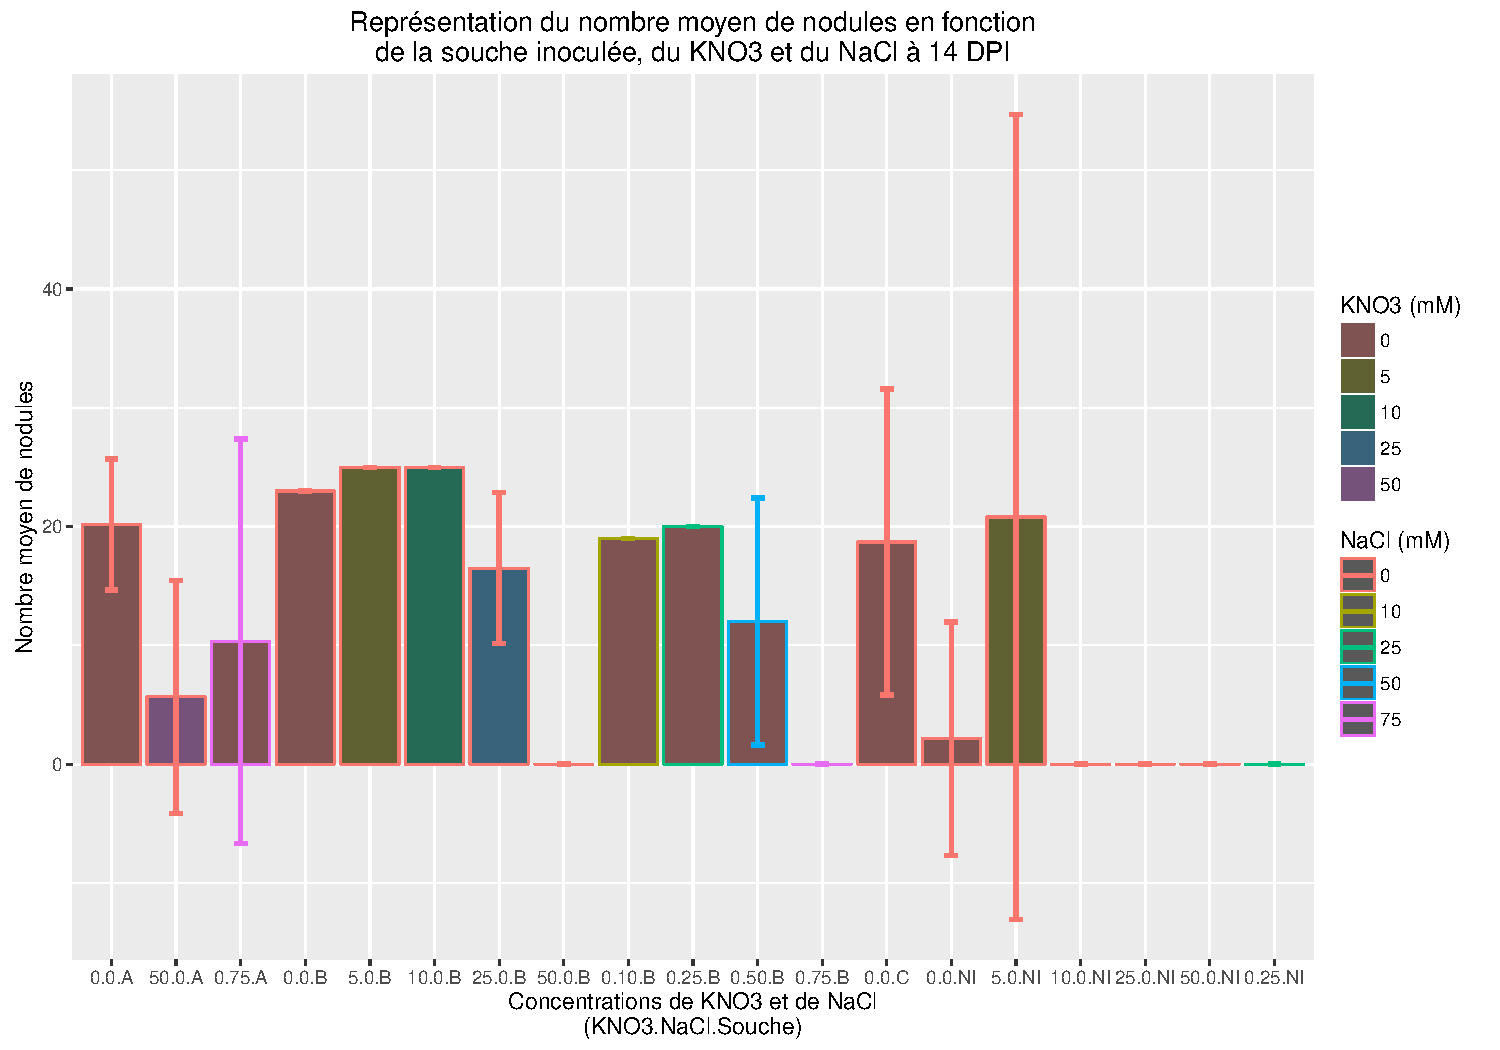
\includegraphics[width=0.9\linewidth]{nodmean14.pdf}
			\end{center}
			\caption{Nombre moyen de nodules en fonction de la souche inoculée, du KNO3 et du NaCl à 14DPI (NI : non inoculée, A, B et C : inoculation avec la souche  A, B et C)}
			\label{nodmean14}
		\end{figure}

		\begin{figure}[p]
			\begin{center}
				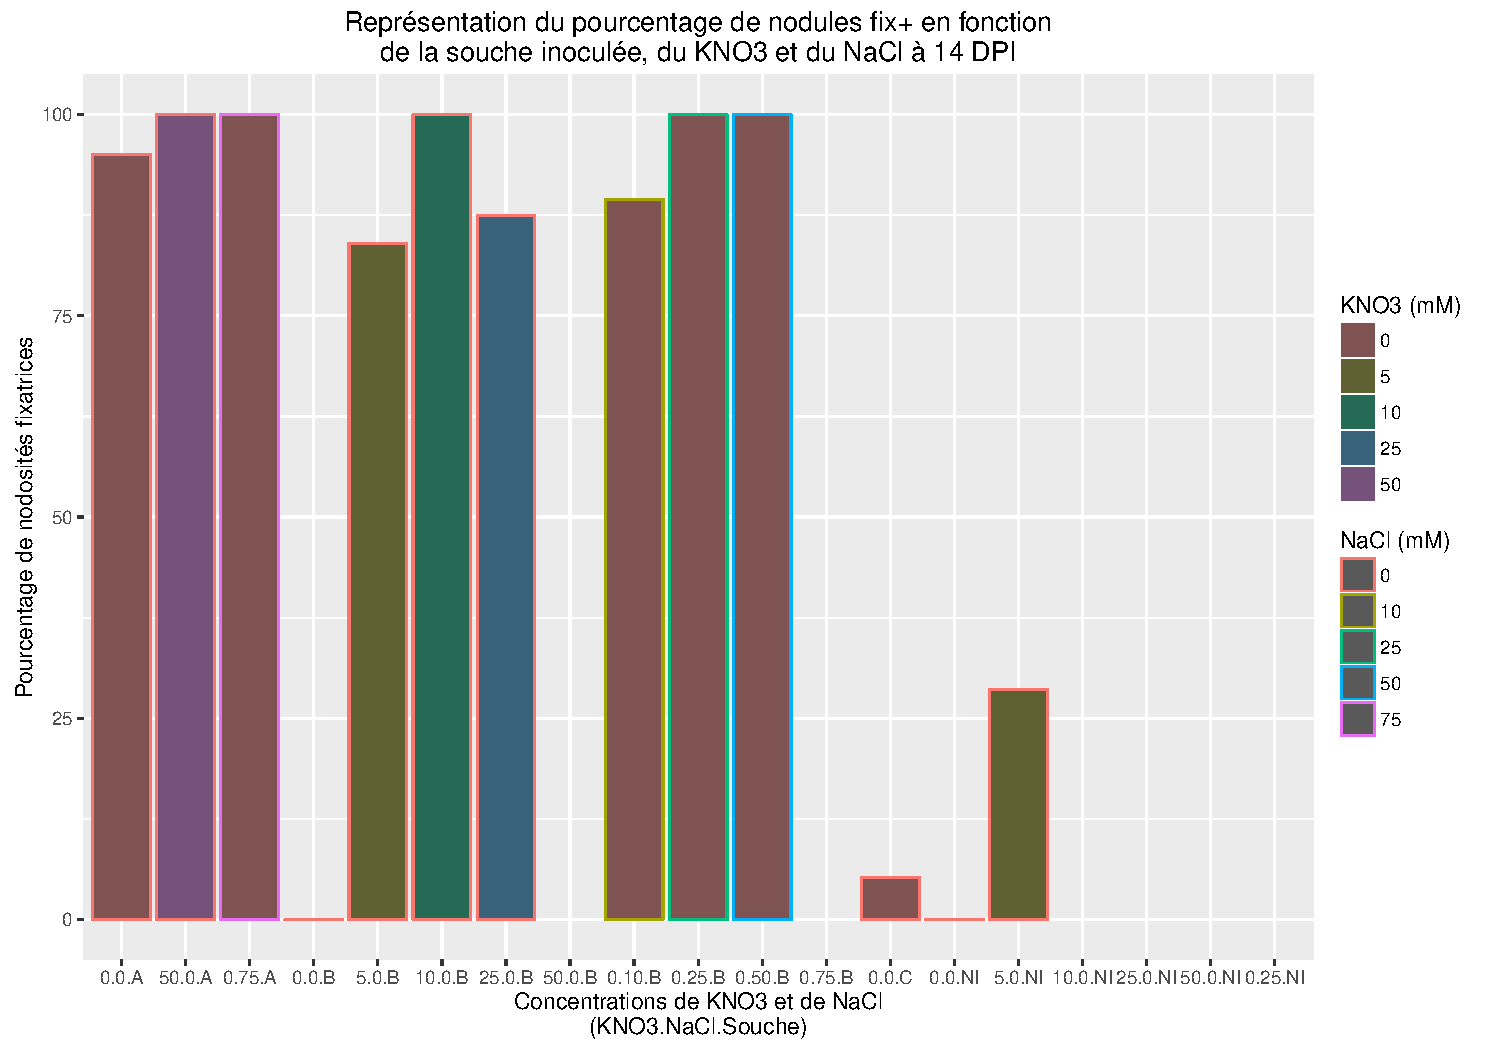
\includegraphics[width=0.9\linewidth]{rapfix+nod14.pdf}
			\end{center}
			\caption{Pourcentage de nodules fixateurs d’azote en fonction de la souche inoculée, de KNO3 et du NaCl à 14 DPI}
			\label{fix+-14}
		\end{figure}




	% \bibliographystyle{unsrt}
	% \bibliography{biblio.bib}


\end{document}
